\subsection{Controlled complete-enumeration measurements}

The retained experiment has 13 geometric cohorts, one warm-up per scope,
and five paired rounds in alternating AB/BA order. The eight-tetrahedron
base with cap type one also has duplicate same-method A/A arms. There are
280 measured calls and 52 warm-up calls across the two scopes, followed by
three new-method-only capacity runs. The immutable predecessor is copied
from the pinned repository revision, rather than recreated by editing the
optimized implementation. Every measured output hash agrees between arms,
and the timed source-file hashes are checked before and after the run.

Table~\ref{tab:enumeration} reports medians in milliseconds. Its speedup is
the median of the five \emph{paired ratios}, which need not equal the ratio
of the two separately reported medians. The last column isolates enumeration
with an already constructed kernel. Full raw calls, order, setup costs,
work counters, and source hashes are in \texttt{results/benchmark.json}.

\begin{table}[htbp]
\centering\small
\begin{tabular}{@{}rrrrrr@{}}
\toprule
$t$ & Cap & Old full (ms) & New full (ms) & Full speedup & Reused speedup\\
\midrule
2 & 1 & 0.626 & 0.425 & 1.51$\times$ & 2.02$\times$\\
2 & 2 & 0.550 & 0.324 & 1.75$\times$ & 2.28$\times$\\
5 & 1 & 8.020 & 1.021 & 7.85$\times$ & 13.88$\times$\\
5 & 2 & 7.516 & 0.993 & 7.70$\times$ & 13.00$\times$\\
9 & 1 & 56.963 & 2.548 & 22.89$\times$ & 41.01$\times$\\
9 & 2 & 75.142 & 2.603 & 30.59$\times$ & 45.10$\times$\\
17 & 1 & 476.595 & 6.921 & 68.86$\times$ & 167.84$\times$\\
17 & 2 & 526.057 & 9.083 & 66.86$\times$ & 171.14$\times$\\
33 & 1 & 6,063.538 & 29.023 & 202.71$\times$ & 781.17$\times$\\
33 & 2 & 6,308.664 & 30.404 & 207.49$\times$ & 728.34$\times$\\
\midrule
9 & 0 & 17.964 & 2.119 & 8.07$\times$ & 17.00$\times$\\
17 & 0 & 98.115 & 7.708 & 12.62$\times$ & 35.20$\times$\\
33 & 0 & 569.414 & 28.207 & 19.75$\times$ & 75.50$\times$\\
\bottomrule
\end{tabular}
\caption{Complete enumeration on capped Fibonacci solid tori. Here
$t=n+1$ includes the cap. ``Full'' includes kernel construction and full
standard-coordinate emission. Types one and two have three rays; type zero
is the two-ray control. Every query has matching nullity two.}
\label{tab:enumeration}
\end{table}

For $t=33$ and cap type one, the old and new full medians are
6.064 seconds and 29.023 milliseconds, with paired speedup $202.71\times$.
The reused-kernel medians are 6.593 seconds and 8.204 milliseconds,
with paired speedup $781.17\times$. These are local complete-enumeration
measurements on the declared family, not whole-recognizer measurements.

The growth in redundant work is also visible without a clock. At base size
$n=32$, the old backend constructs 35 distinct hyperplanes, tries 34
nonnegative directions, and rejects 31; the new method lifts precisely three
directions. Corollary~\ref{cor:oldfamily} proves these counts for every
size. The timing difference also includes the cost of constructing pairwise
forms and applying dense supported-rank tests, so it should not be explained
only by the ratio of candidate counts.

The same-method duplicate ratios (first call divided by duplicate) have medians 0.969 and 0.974 for reused old/new calls, and 0.794 and 1.037 for full old/new calls. This visible host variability argues against treating small differences or last decimal places as reliable. No confidence interval or power-law fit is claimed.


\begin{table}[htbp]
\centering\small
\begin{tabular}{@{}rrrrr@{}}
\toprule
$t$ & Kernel (ms) & Enumeration (ms) & Total (ms) & Kernel share\\
\midrule
65 & 126.833 & 28.028 & 154.861 & 81.9\%\\
129 & 926.795 & 144.873 & 1,071.667 & 86.5\%\\
257 & 7,493.208 & 395.727 & 7,888.936 & 95.0\%\\
\bottomrule
\end{tabular}
\caption{New-method-only capacity runs with cap type one and three emitted
rays. Each row is a single call, not a paired comparison or a median.}
\label{tab:capacity}
\end{table}

At $t=257$, approximately 95\% of the new full call is kernel construction.
This identifies a concrete implementation target after removing arrangement
work. The capacity rows do not imply a measured speedup at these sizes:
the predecessor was not run there.

\begin{figure}[htbp]
\centering
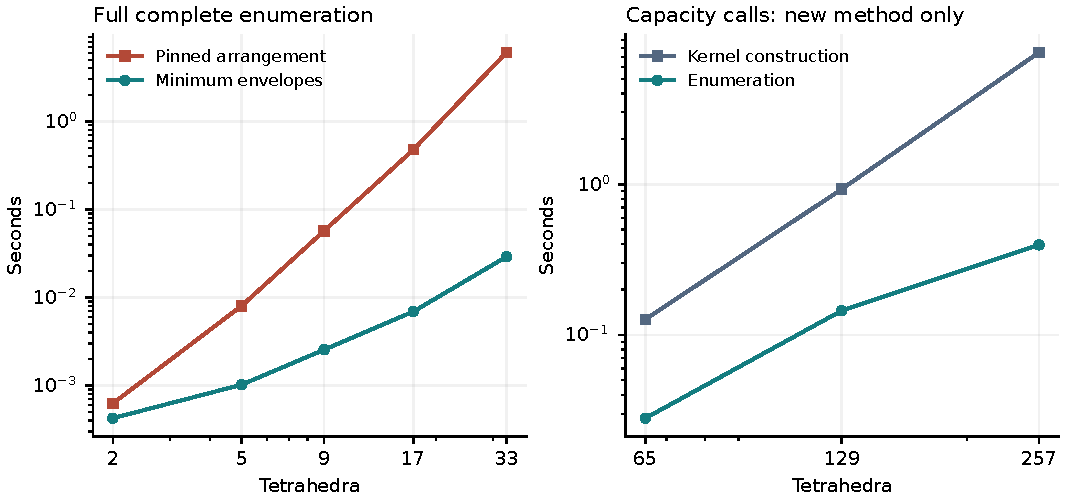
\includegraphics[width=\linewidth]{figures/measurements.pdf}
\caption{Measured complete-enumeration times. Left: five-round medians of
full calls on cap-type-one inputs, including kernel construction. Right:
the three new-method-only capacity calls, separated into kernel and
enumeration time. Both axes in each panel are logarithmic. Lines connect
observations and are not fitted complexity laws.}
\label{fig:measurements}
\end{figure}

\subsection{Production followed by independent coverage checking}

A separate matched workflow includes completeness checking. The old arm
constructs the pinned kernel, enumerates with the pinned arrangement, then
reconstructs the independent dense matching model and runs its complete
reference enumeration to check equality. The new arm produces an envelope
coverage certificate and replays it with the independent uncontracted-graph
checker. Both workflows require the same complete ray list. The new API
constructs its plan for both production and certification; this duplicate
constant-factor work is included in the timings.

There is one warm-up and three paired AB/BA rounds for each compared size.
Fixture generation and final reporting serialization and hashing are outside
the timed regions. The old arm's ray-list equality check and the new arm's
certificate verification, including their internal hashes, are included.
\texttt{results/coverage.json} retains every call, source hash, and six
independently replayable source/certificate pairs.

\begin{table}[htbp]
\centering\small
\begin{tabular}{@{}rrrr@{}}
\toprule
$t$ & Old production + replay (ms) & New production + replay (ms) & Paired speedup\\
\midrule
2 & 1.713 & 1.010 & 1.68$\times$\\
9 & 130.931 & 8.628 & 15.18$\times$\\
17 & 1,326.585 & 29.259 & 51.92$\times$\\
\bottomrule
\end{tabular}
\caption{Complete production and independent coverage, cap type one.
Reported times are medians; speedups are medians of paired ratios.}
\label{tab:coveragebench}
\end{table}

\begin{table}[htbp]
\centering\small
\begin{tabular}{@{}rrrrrr@{}}
\toprule
$t$ & Production (ms) & Replay (ms) & Total (ms) & Certificate bytes & Tests\\
\midrule
33 & 43.729 & 53.800 & 97.529 & 3,915 & 132\\
65 & 248.320 & 328.658 & 576.978 & 9,985 & 260\\
129 & 1,616.358 & 2,322.612 & 3,938.970 & 29,654 & 516\\
\bottomrule
\end{tabular}
\caption{New-only production and coverage capacity calls. ``Tests'' counts
slope-bracket dominance checks, exactly $4t$ per row. Each list has three
rays. JSON sizes include the complete coordinates; serialization is untimed.}
\label{tab:coveragecapacity}
\end{table}

The coverage workflow at $t=17$ has median paired speedup $51.92\times$;
its three ratios range from $34.61\times$ to $60.72\times$. This broader
scope shows that the benefit persists after checking a complete answer.
At $t=129$, new production and replay take a single combined 3.939 seconds;
this is a capacity observation without a comparative claim. The $4t$
dominance count does not imply a linear-time full checker, since matching
elimination, projection, and coordinate validation must also be performed.

